\chapter{驱动程序的设计和实现}
	
	设备驱动程序在操作系统中框架是操作系统的设计人员在设计操作系统时已经制定好的,	所以在进行驱动程序的开发时需要开发人员对操作系统和设备的硬件体系具有相当的了解,而且驱动程序的性能、可靠性也制约着系统的性能和可靠性。	


\section{VxWorks上的USB开发}
	在VxWorks当中I/O框架的实现放在内核文件ioLib.c当中,我们将它称为上层接口子系统,因为它负责给上层应用提供I/O接口,但是该接口并不会完成具体请求的实现,他只会在进行简单的处理之后将请求转发给I/O子系统,具体请求的处理工作会被发送到I/O子系统当中来处理。I/O子系统的定义放在在内核文件iosLib.c当中,I/O子系统对用户层而言通常是透明的,用户层一般不会直接调用I/O子系统中的函数,它是作为上层接口子系统与下层驱动系统的中间层来使用的。VxWorks的当中内核驱动层次结构如\autoref{fig:VxWorks内核驱动层次结构}所示。	

\begin{figure}[!h]
\centering
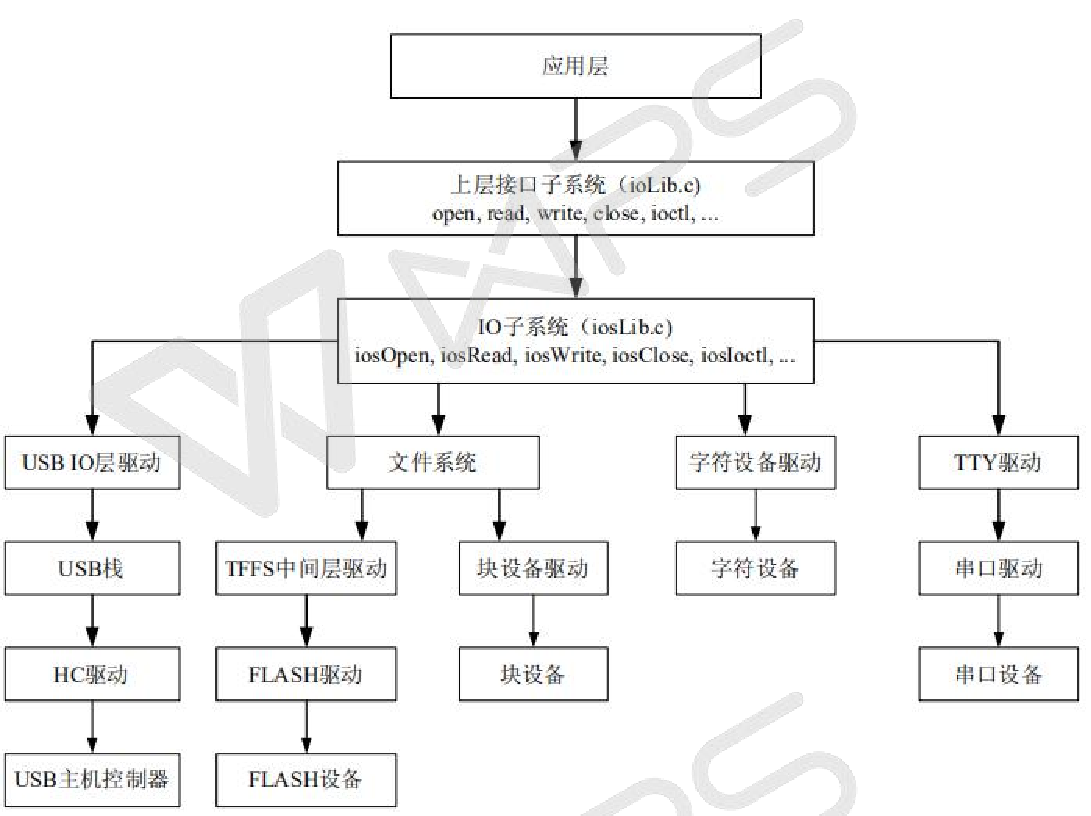
\includegraphics[width=0.9\textwidth]{./graphics/vxworks-kernel-diagram.pdf}
\caption{VxWorks驱动内核层次结构}\label{fig:VxWorks内核驱动层次结构}
\end{figure}	
			
	从\autoref{fig:VxWorks内核驱动层次结构}当中我们可以看出USB驱动在VxWorks当中的层次结构,		
	在VxWorks当中USB驱动程序堆栈的开发符合的是通用串行总线规范2.0标准,VxWorks中的将USB协议在主机端分成三层来实现,分别是客户端驱动程序(Client Driver)、USB驱动(USBD)、主机控制器驱动(HCD),每一层完成不同的功能。其通信的逻辑结构和PC端的软硬件结构如\autoref{fig:USB通信结构}所示。
\begin{figure}[h]
\centering
  \begin{subfigure}[b]{0.4\textwidth}
  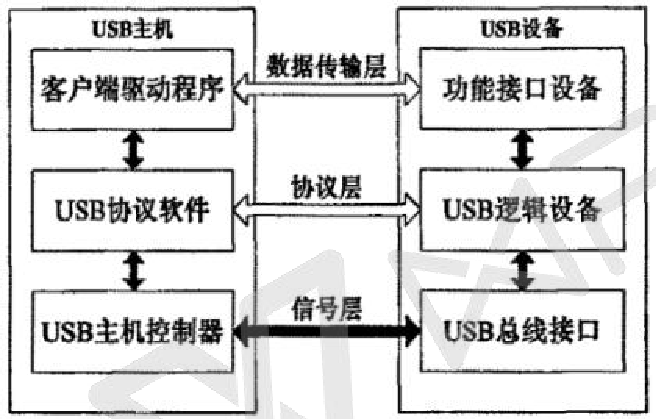
\includegraphics[width=1.0\textwidth]{./graphics/USB-device-structure-diagram.pdf}
  \caption{USB通信的逻辑结构}\label{fig:usb通信逻辑结构}
  \end{subfigure}
  ~
  \begin{subfigure}[b]{0.5\textwidth}
  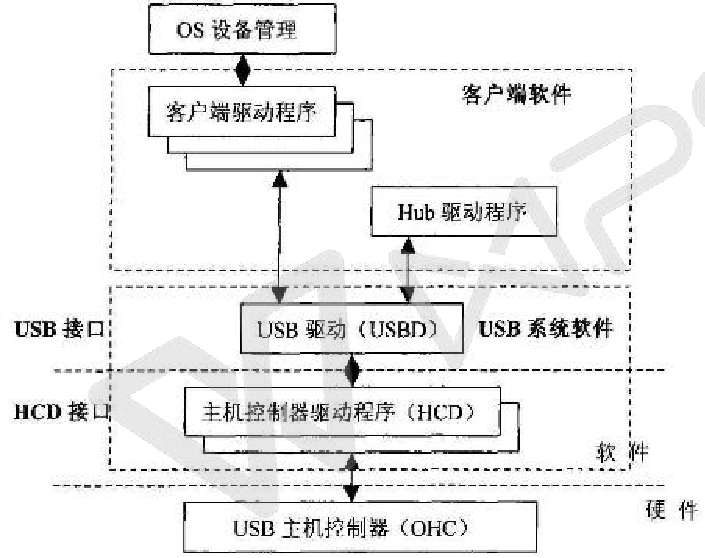
\includegraphics[width=1.0\textwidth]{./graphics/USB-PC-structure.pdf}
  \caption{USB主机端软硬件结构}\label{fig:usb-PC}
  \end{subfigure}
\caption{USB通信结构}\label{fig:USB通信结构}
\end{figure}
	
	客户端驱动程序的功能是完成对不同类型设备的功能驱动。本次设计中所要完成的USB口转串口的驱动要完成的就是客户端驱动。USB口转串口驱动会构建USB I/O请求包(I/O request,IRP)来向USBD层发出数据接收或者发送的请求,IRP是USB协议中定义的一个抽象概念,我们需要根据所发送的内容和发送的方式来具体的实现一个IRP\cite{李雪红2004USB}。
	
	USBD是USB的核心驱动,其提供了操作系统组件(主要是设备驱动)能够用来访问USB设备的方法,其实现是由操作系统决定的。USBD提供包括USB总线的枚举、总线带宽的分配、传输控制等操作,它还会处理客户端驱动程序发送来的IRP包,并在对IRP请求包进行解析之后将实际的请求映射到适当的HCD或者直接交给主机控制器处理。除此之外USBD负责的内容还包括新设备的动态插拔、电源管理和对客户端驱动程序的维护等。
	
	HCD层提供一个软件抽象来完成USB主控制器的各种事物处理,用于隐藏主控制器的硬件实现细节,HCD只服务于我们的USBD层,对上层应用而言其通常是不能直接访问的。HCD层会将USBD层传输下来的事务调度给主机控制器进行处理,当事物处理完成之后HCD层会将处理结果返回给USBD层。此外它还会完成对主机控制器和根集线器的配置和驱动等操作\cite{李雪红2004USB}。
	
	对于我们的USB口转串口驱而言,我们不再需要实现对物理设备的数据结构抽象,因为VxWorks中的USB HCD层已经为我们实现好了物理层的抽象,同时还给我们提供了USBD层,因此我们只需要实现USB主机三层结构当中的客户端驱动程序即可,使其能够驱动特定的USB设备正常工作。在客户端驱动当中,我们需要完成IO系统的各类接口的实现、完成驱动需要实现的特殊功能的实现、将驱动集成到系统中等工作。
	


\section{CP2102开发}
	除了驱动程序之外,USB口转串口的实现还需要硬件来作为支撑,PC机上本身并没有USB/RS-232的转换器,
	对于USB/RS-232转换器的设计通常有两类实现方式:一类是使用包含有USB单元的微处理器从底层的硬件和固件进行全面系统的设计,这样的控制器有PCI16C745、68HC705JB4和C541U系列等\cite{USB与RS232接口转换器的设计},但是使用这种方式从头开始设计存在难度大,系统复杂等问题,不符合我们本次设计工作的需求。
	第二类方法是采用市场上设计好的USB/RS-232双向转换芯片,这类芯片有CH341,CP2102、FT232BM等,我们在此处的设计即使用了CP2102芯片作为USB/RS-232转换器,这样设计的好处是不需要编写转换器芯片的固件,节约开发时间,由于这个技术已经很成熟,大多的USB口转串口的解决方案都会采用这种已经设计好的集成芯片来作为转换器。
	
	CP2102是SILICON LABORATORIES推出的USB与RS232接口转换芯片,
	它包含有一个USB2.0全速功能控制器,EEPROM,USB收发器,振荡器和异步串行数据总线(UART),在SILICON给出的文档当中已经帮我们给出了一个最简单 CP2102的使用方式的电路框图,如\autoref{fig:cp2102电路框图}所示。
\begin{figure}[!h]
\centering
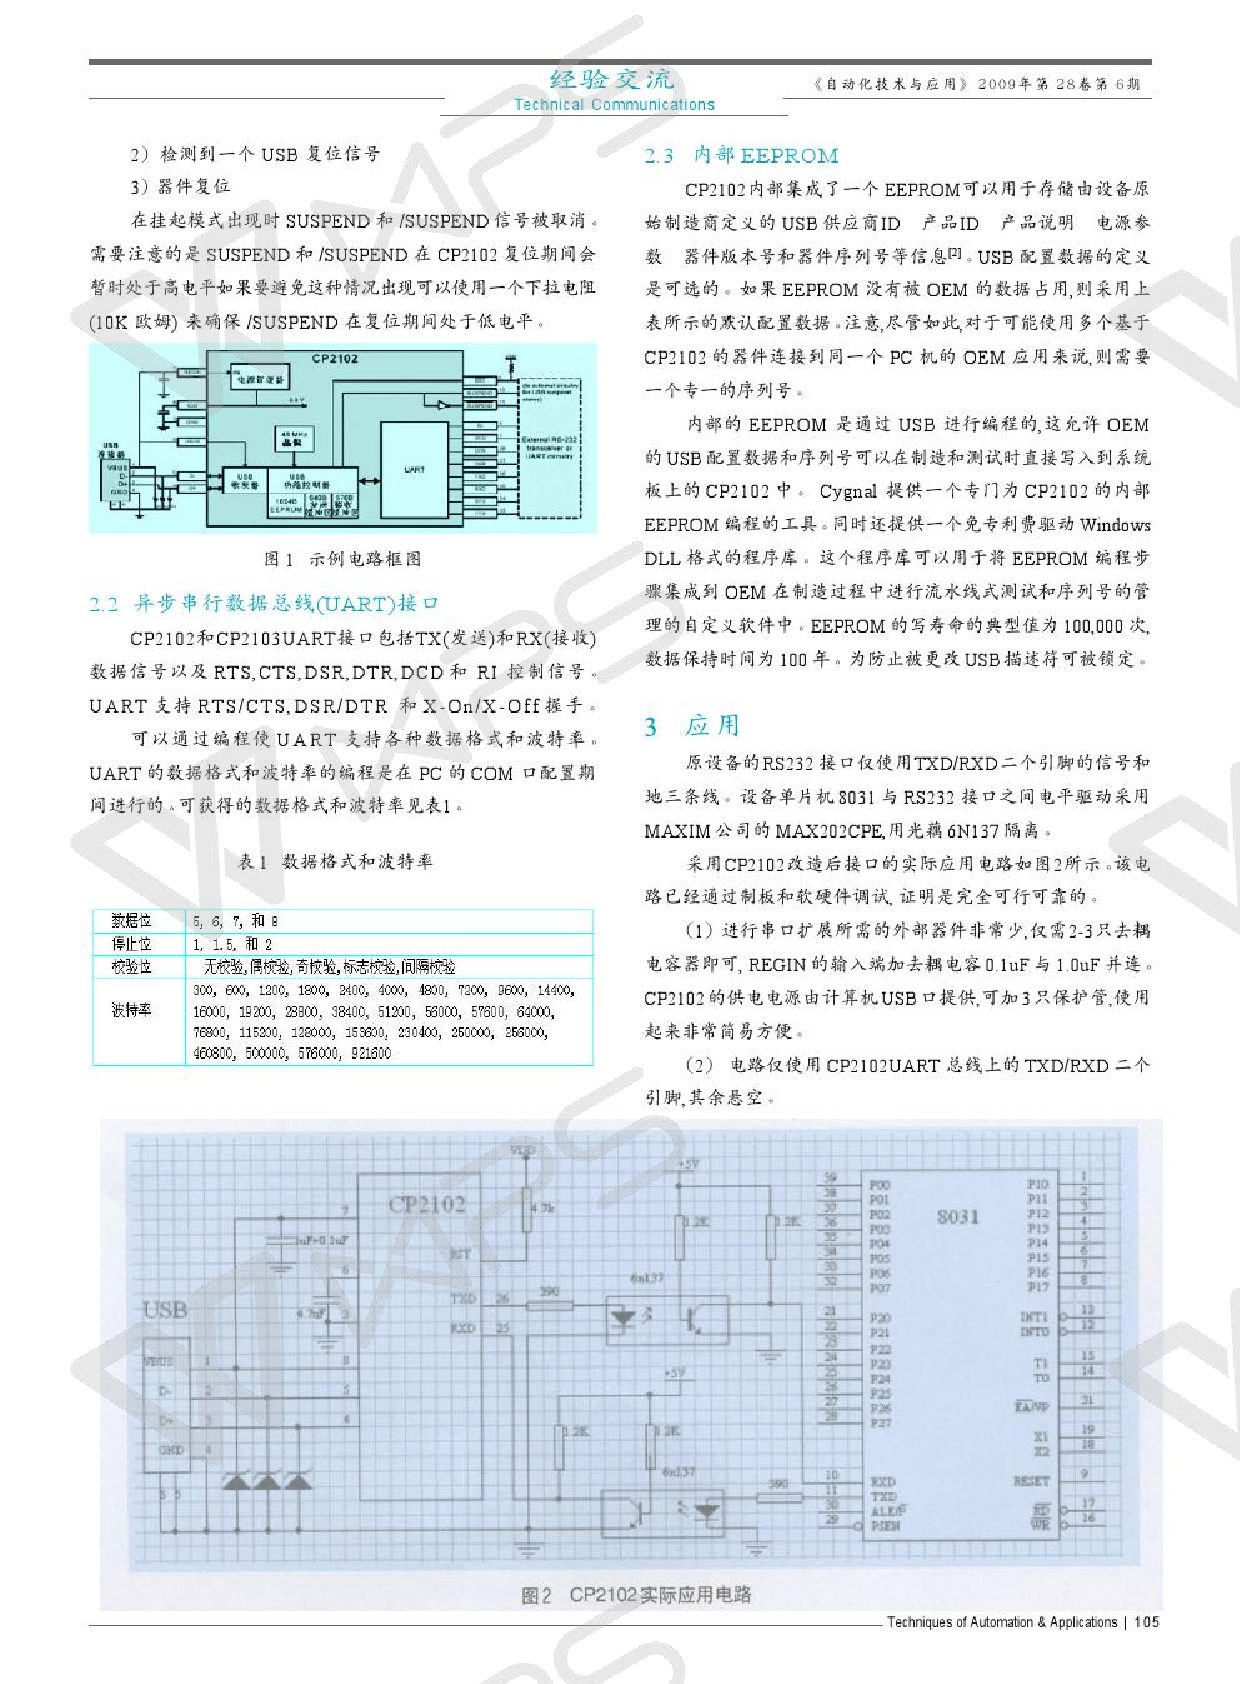
\includegraphics[width=1.0\textwidth]{./graphics/cp2102-circuit-diagram.pdf}
\caption{cp2102电路框图}\label{fig:cp2102电路框图}
\end{figure}

\begin{enumerate}
\item CP2102的USB功能控制器和收发器:CP2102的内置的USB功能控制器符合USB2.0协议,它负责管理USB和UART之间的所有数据和控制传输。
\item 异步串行数据总线(UART)接口:CP2102的UART接口支持接收、发送、控制、握手信号,而且支持对UART数据格式和波特率进行编程控制。可以使用的数据格式和波特率见\autoref{fig:CP2102可配置参数}。
\item 内部EEPROM:CP2102内部集成了一个1K的BEEPROM,在其中存储了一些设备的特定信息,包括厂商ID、产品ID、产品说明、电源参数、器件版本号和器件序列号等\cite{CP2102}。如果OEM没有为设备的EEPROM写入数据的话,那么设备会自动的使用一组默认的数据,如\autoref{CP2102DefaultConfigure}所示。
\end{enumerate}

\begin{figure}[!h]
\centering
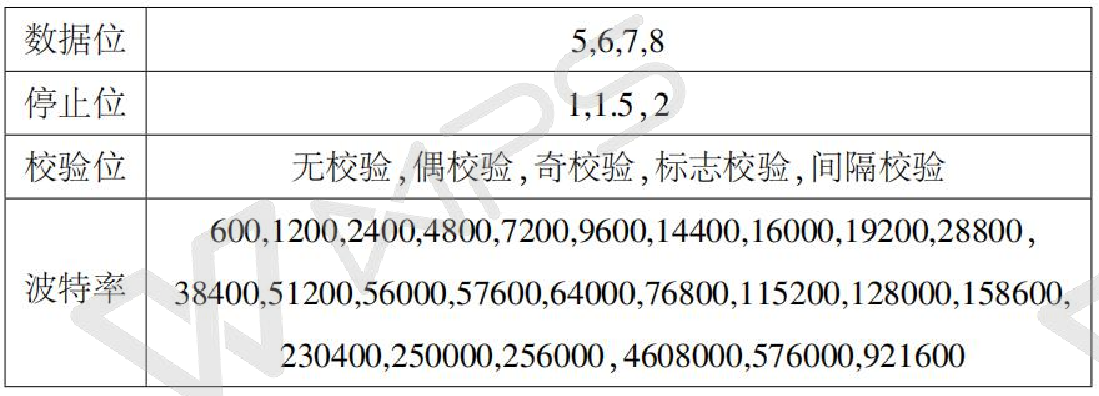
\includegraphics[width=1.0\textwidth]{./graphics/CP2102ChioceConf.pdf}
\caption{cp2102可选配置参数}\label{fig:CP2102可配置参数}
\end{figure}

\begin{figure}[!h]
\centering
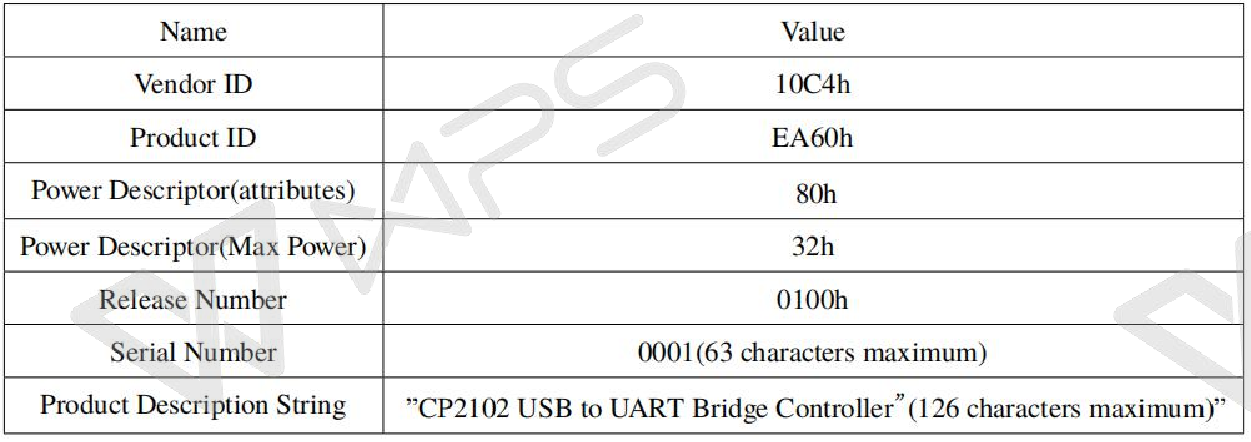
\includegraphics[width=1.0\textwidth]{./graphics/CP2102DefConf.pdf}
\caption{CP2102默认配置表}\label{CP2102DefaultConfigure}
\end{figure}
	使用CP2102进行串口扩展的时候只需少量外部器件,
	CP2102当中的协议控制单元会对来自USB接口的命令进行解析,然后对UART接口进行配置。UART的部分可配置参数如\autoref{fig:CP2102可配置参数}所示,
	CP2102当中的拥有一个576B的接收缓冲区和一个640B发送缓冲区,这些缓冲区可以部分的解决USB和RS-232之间的速率不匹配的问题。以从计算机到外设的数据传输为例。当USB转串口设备连接到PC的USB总线上后,PC会对其进行初始化并在识别出该设备后启动支持该设备的客户端驱动;计算机上的驱动程序会将数据包传输给USB接口(通常使用批量传输的方式),设备从USB接口提取出数据并保存在数据缓冲区中,UART接口再从数据缓冲区中将数据取走并发送出去,从外设传输数据到计算机的方式则相反\cite{李雪红2004USB}。	
	
	在我们本次的设计当中我们并不会去完成CP2102的外部电路的设计工作,而是选择市场上已经封装好的模块。我们本次使用的设备如\autoref{fig:cp2102模块正反面}所示。我们所需要做的是了解CP2102的原理和功能,能够对其进行正确的开发工作。
\begin{figure}[h]
\centering
  \begin{subfigure}[b]{0.4\textwidth}
  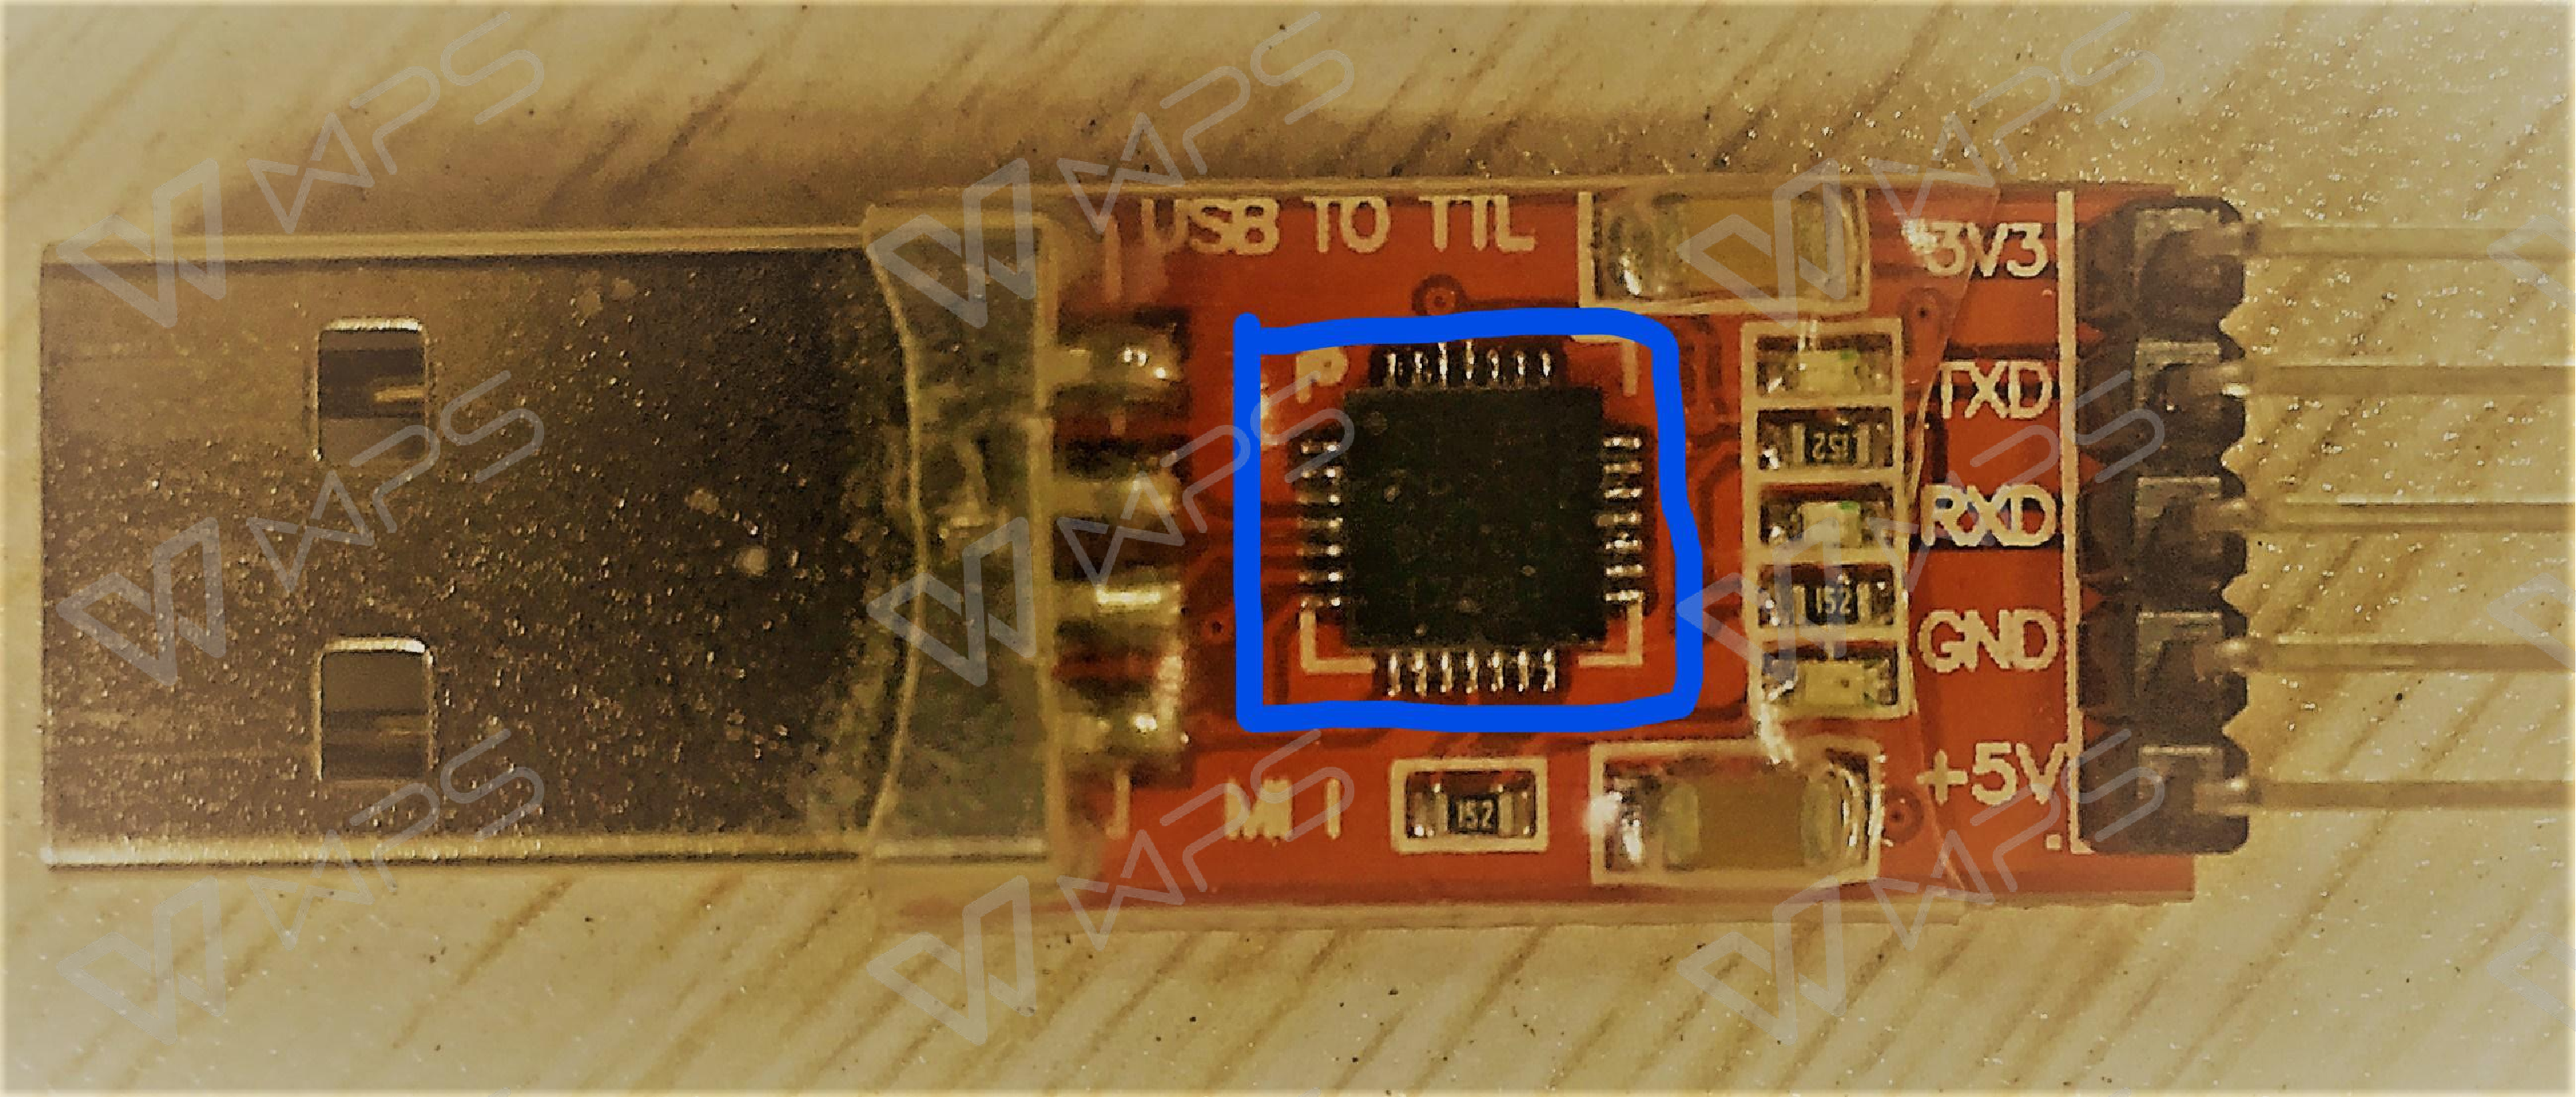
\includegraphics[width=\textwidth]{./graphics/cp2102Front.pdf}
  \caption{CP2102模块正面}\label{fig:cp2102Front}
  \end{subfigure}
  ~
  \begin{subfigure}[b]{0.4\textwidth}
  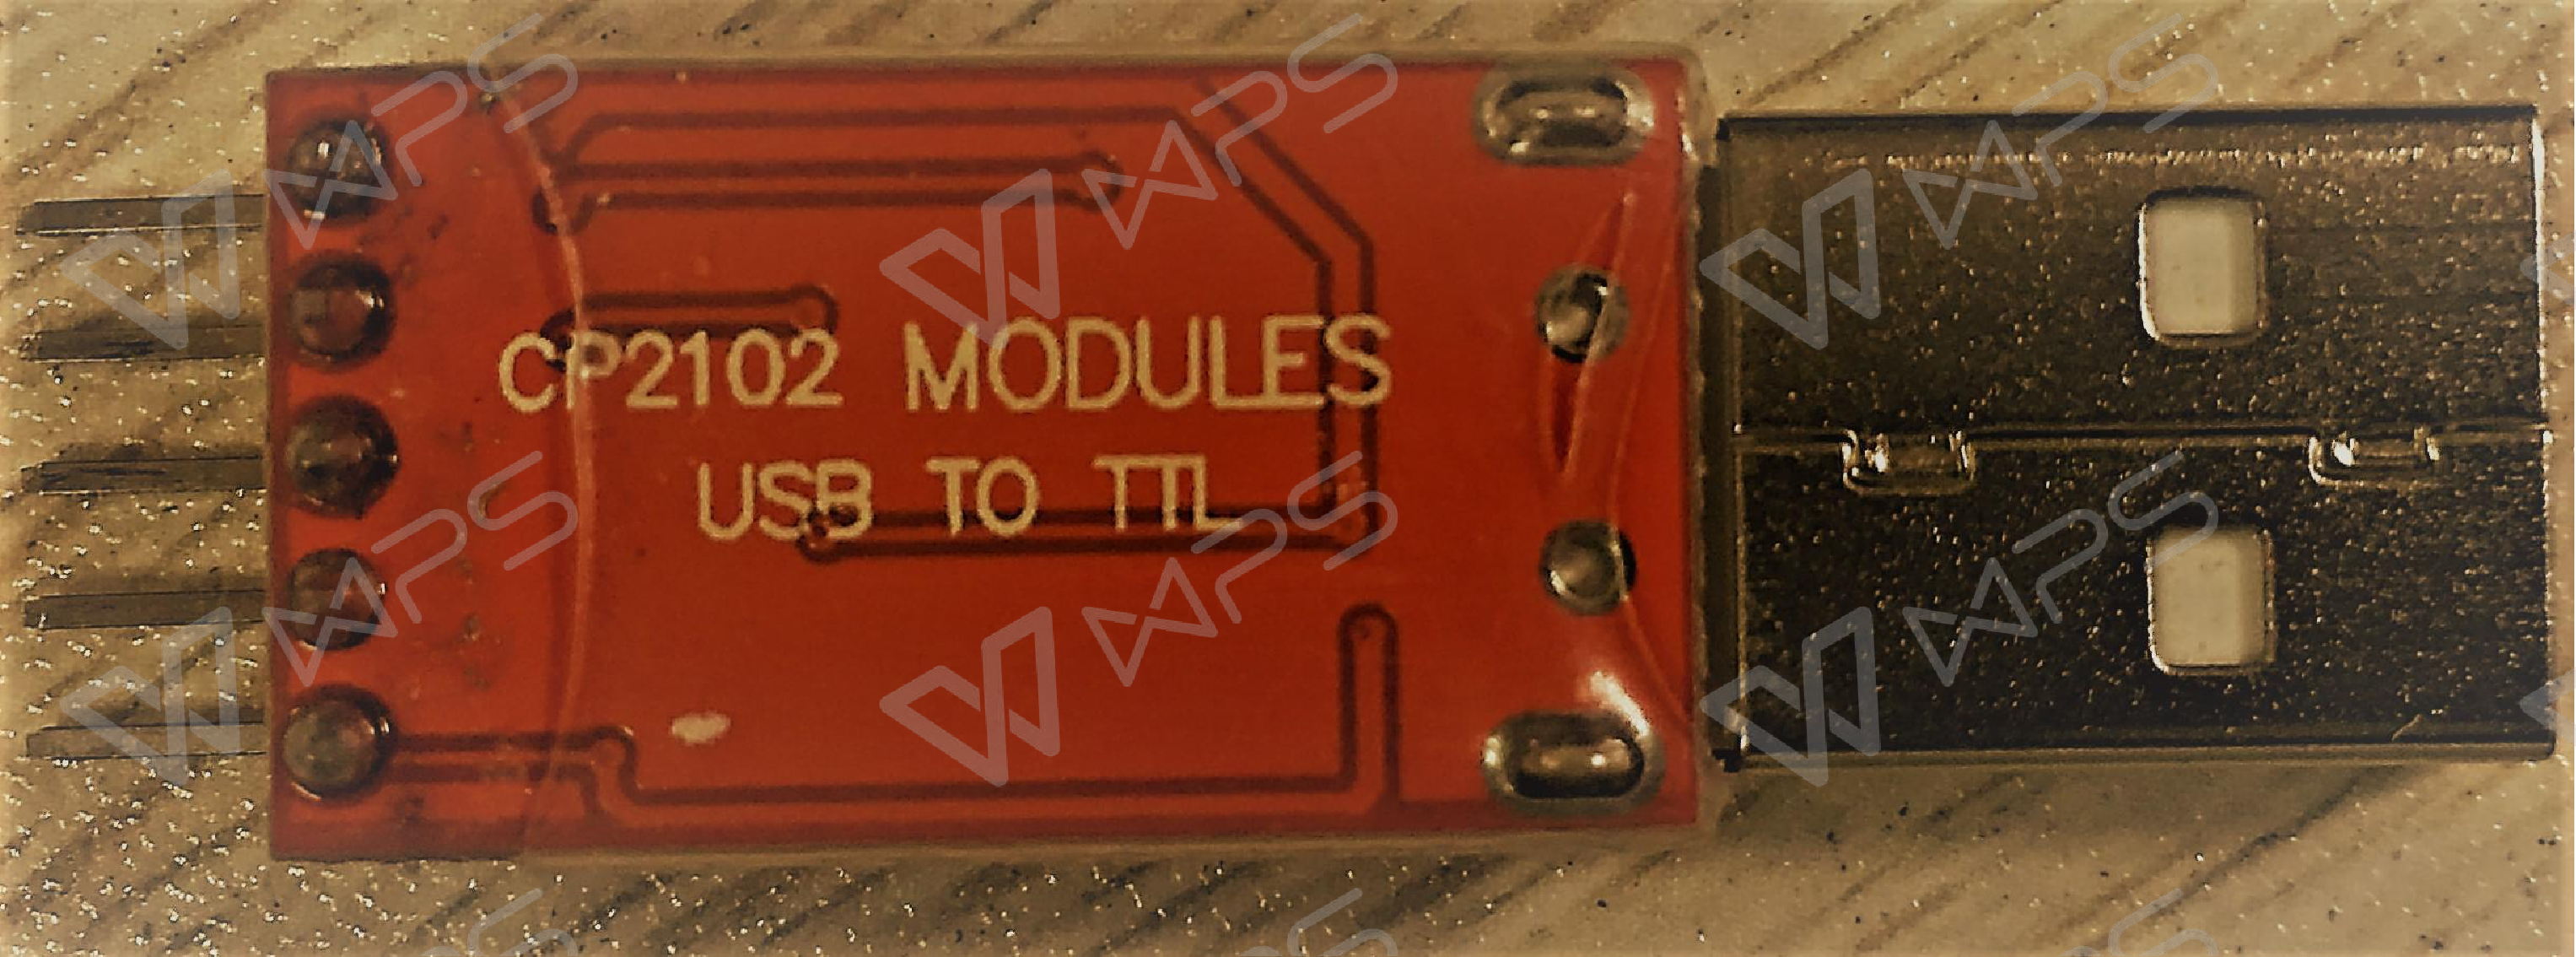
\includegraphics[width=\textwidth]{./graphics/cp2102Rear.pdf}
  \caption{CP2102模块反面}\label{fig:cp2102Rear}
  \end{subfigure}
\caption{CP2102模块正反面}\label{fig:cp2102模块正反面}
\end{figure}
	

\section{特定需求单设备驱动的实现}

	
	在VxWorks I/ O 当中通常应该经过以下的三个基本步骤来实现一个设备驱动:
\begin{enumerate}
\item 实现对实际物理设备的数据结构抽象(即设备的自定义数据结构);
\item 完成 I/ O 系统所需要的各类接口及自身的特殊接口(open、read、write等);
\item 将驱动集成到操作系统中。
\end{enumerate}

	无论驱动程序的开发人员要完成一个什么样的驱动程序,其都有一些系统规定的标准的模块,以方便控制设备。我们此次驱动程序需要实现的框架部分主要包括cp210xDrvInit()、cp210xDevOpen()、cp210xDevClose()、cp210xDevIoctl()、cp210xDevWrite()、cp210xDevRead()、cp210xDrvUnInit()等函数,如\autoref{lab:驱动程序的关键模块}所示 ,在这些模块当中关键要处理的内容是对数据的传输工作和对设备的控制工作,数据的传输要用到缓冲区和用于进行同步和互斥操作的信号量。
\begin{table}[!h]
\centering
\begin{tabular}{|c|c|}
\hline
{模块} & {作用} \\
\hline
{cp210xDrvInit()} & \tabincell{c}{这个模块用来初始化驱动程序,主要是与设备无关的一些\\全局变量并向系统注册该驱动} \\
\hline
{cp210xDevOpen()} & \tabincell{c}{这个模块用来转接I/O子系统分发过来的open()操作,实现设备的打开,\\返回文件描述符} \\
\hline
{cp210xDevClose()} & \tabincell{c}{这个模块用来转接I/O子系统分发过来的close()操作,实现设备的关闭,\\对设备占用资源进行清理} \\
\hline
{cp210xDevIoctl()} & \tabincell{c}{这个模块用来转接I/O子系统分发过来的ioctl()操作,\\实现对设备的一些特定的控制操作} \\
\hline
{cp210xDevWrite()} & \tabincell{c}{这个模块用来转接I/O子系统分发过来的write()操作,\\实现对设备进行数据的写入} \\
\hline
{cp210xDevRead()} & \tabincell{c}{这个模块用来转接I/O子系统分发过来的read()操作,\\用于从设备读取数据。} \\
\hline
{cp210xDrvUnInit()} & \tabincell{c}{这个模块用来卸载驱动程序,将驱动从系统驱动表中删除,\\并清理该驱动程序所占用的全部资源} \\
\hline
\end{tabular} 
\caption{驱动程序的关键模块}\label{lab:驱动程序的关键模块}
\end{table}


	由于对于仅支持单设备驱动程序是基于特定的需求而具体定制的,所以该设备的驱动程序的实现流程与通常的支持多设备的驱动的初始化流程存在差异。具体的需求为:\\
\hei{1. 驱动中支持的设备名是固定的,无论具体的设备是否连接上,都可以往这个设备中写入数据。}\\
\hei{2. 驱动程序中要有缓存一定数据的能力,一旦设备连接之后就能够检查缓冲区中是否有数据,有数据则将其发送出去。}

	由于需要在设备未连接时就能够往设备中写入数据,且设备名为固定的,那么就必须调整驱动的初始化流程,使得其能够支持这一特性,通常驱动都是在设备加载之后再将其加入到系统设备表和系统驱动表当中,那么此时我们就需要先将一个固定的设备名加入到系统设备表当中。对于该特定需求的单设备驱动的流程图如\autoref{fig:SDev-Drv-diagram}和所示。
\begin{figure}[h]
\centering
  \begin{subfigure}[b]{1.0\textwidth}
  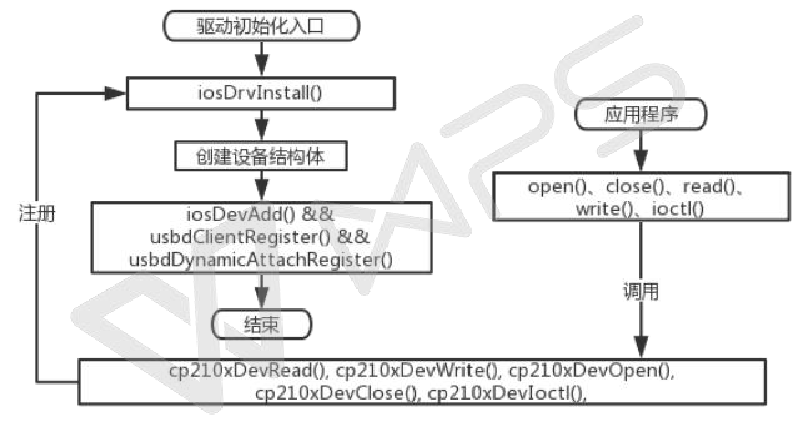
\includegraphics[width=\textwidth]{./graphics/SDev-Drv-Diagram-a.pdf}
  \caption{}\label{fig:SDevice-Driver-diagram-a}
  \end{subfigure}
  ~
  \begin{subfigure}[b]{1.0\textwidth}
  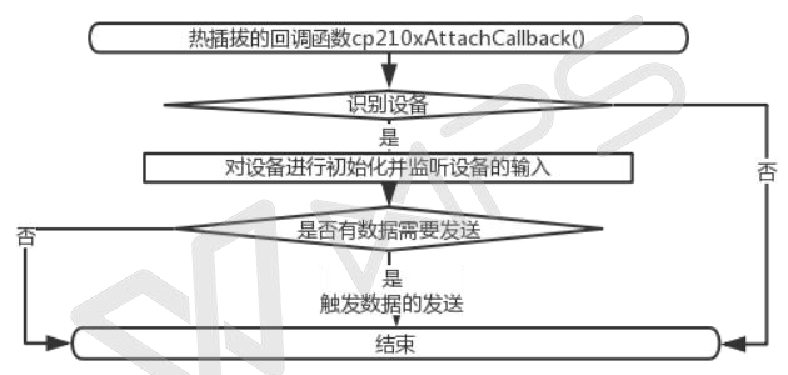
\includegraphics[width=\textwidth]{./graphics/SDev-Drv-Diagram-b.pdf}
  \caption{}\label{fig:SDevice-Driver-diagram-b}
  \end{subfigure}
\caption{特定需求单设备驱动运行流程图}\label{fig:SDev-Drv-diagram}
\end{figure}




\subsection{设备的自定义结构}
	底层驱动都要对其驱动的设备维护一个自定义的数据结构,这个结构的第一个成员必须是
	DEV\_ HDR结构体,其余的成员为该设备所需的关键参数。对于我们的USB口转串口设备需要保存的关键参数有:USB配置、读写缓冲区的指针、接口配置、端点地址等等。关键数据结构的定义如下: 
	
\lstset{language=C}
\begin{lstlisting}
typedef struct cp210x_dev
{
  DEV_HDR cp210xDevHdr; 
  
  UINT16 numOpen;
  USBD_NODE_ID nodeId;
  UINT16 configuration;	
  UINT16 interface; 
  UINT16 interfaceAltSetting;
  UINT16 vendorId;
  UINT16 productId;

  BOOL connected;  
  int trans_len;
  USBD_PIPE_HANDLE outPipeHandle; 
  USB_IRP	outIrp; 
  BOOL outIrpInUse; 
  UINT16  outEpAddr;
  UINT8 trans_buf[64];

  USBD_PIPE_HANDLE inPipeHandle;
  USB_IRP inIrp;
  BOOL inIrpInUse;
  UINT8 inBuf[64];
  UINT16 	inEpAddr;
} CP210X_DEV, *pCP210XDEV;
\end{lstlisting}
\noindent 部分成员的含义如下:

\begin{itemize}
\item DEV\_ HDR:这一成员必须是自定义设备结构的第一个成员,VxWorks 的I/O子系统会把所有的设备结构都看作是这个类型的结构,wind只会识别到DEV\_ HDR结构并对其进行管理,在系统的设备列表中,内核只使用DEV\_ HDR结构当中的成员。
\item numOpen:用来记录设备被打开的次数,每次调用open()函数打开该设备则numOpen加一,调用close()函数关闭设备则减一。
\item nodeId:用来保存该设备在系统中的唯一ID号。
\item configure、interface、interfaceAltsetting:用来保存设备的描述符中的配置、接口、可变接口信息。
\item vendorId、productId:保存该设备的厂商ID和产品ID,用来识别该设备是否适合我们的驱动程序。
\item outPipeHandle、inPipeHandle:设备的输入/输出端点的管道句柄,每次传输数据时都需要使用该句柄来表明数据传到的哪一个端点。
\end{itemize}






\subsection{驱动注册和设备创建} 
	
	底层的驱动程序都要提供一个函数给系统来调用,以便进行驱动程序的注册和初始化,这些工作的完成通常是在内核启动过程中进行的(即内核启动的时候会调用我们的驱动初始化函数)。对于此处的USB口转串口驱动我们定义cp210xDrvInit() 初始化函数,其主要完成驱动所需要的资源申请和系统的初始化,包括创建信号量、向系统注册驱动、创建设备、向USBD层注册。cp210xDevInit模块主要代码如下所示:
\lstset{language=C}
\begin{lstlisting}
STATUS cp210xDrvInit(void)
{
  ... 	
  cp210xDrvNum = iosDrvInstall(NULL,NULL,cp210xDevOpen,cp210xDevClose,
			cp210xDevRead,cp210xDevWrite,cp210xDevIoctl);
  ...
  if( iosDevAdd(&pCp210xDev->cp210xDevHdr,CP210X_NAME,cp210xDrvNum) != OK)
  ...  
  if(usbdClientRegister (CP210X_CLIENT_NAME, &cp210xHandle) != OK)
  ...  
  if(usbdDynamicAttachRegister(cp210xHandle,USBD_NOTIFY_ALL,USBD_NOTIFY_ALL,USBD_NOTIFY_ALL,TRUE,(USBD_ATTACH_CALLBACK)cp210xAttachCallback)!= OK)
  ...
}
\end{lstlisting}\\

	驱动会在进入初始化的时候首先检查该驱动是否已经安装,若已经安装了则无需再次安装,直接退出即可,cp210xDrvInit()通常是在usrRoot(usrConfig.c)中调用,但是你也可以手动调用这个函数对该驱动进行初始化操作。然后会进行一些驱动所需要的全局资源的初始化,如信号量、全局变量、看门狗等,接着调用iosDrvInstall()函数安装驱动的I/O函数,将其添加到驱动表当中,在我们的USB口转串口驱动当中不需要实现delete函数和create函数,直接将其指针置为NULL即可。
	
	注册完成之后还要向系统将该驱动程序添加到IO子系统当中,添加成功后会在系统的设备列表中显示该命名为CP210X\_ NAME的设备(CP210X\_ NAME只是一个宏定义,设备名可以自己更改)。此处即是我们的驱动程序中的一个特殊的地方,在没有识别到设备之前就已经创建好设备文件,只不过此时该设备还只是一个“假”的,只有软件实现,没有硬件支撑,即使此时已经可以打开该设备,向该设备写入数据,但是也只是写入到了系统的缓冲区当中而已,数据并没有发送到任何的硬件上。

	接下来USB客户端驱动还需要向USBD层注册,注册完成之后会返回一个用于操作USBD的客户端handle,我们将其保存在cp210xHandle这个变量当中。然后还要注册一个动态注册的回调函数,当USBD层发现有USB设备的插拔动作时,就会根据我们注册时选定的设备类和接口类来判断是否需要调用我们注册的回调函数,由于我们的设备是一个特殊的设备,并不符合任何标准的USB设备类和接口类,于是我们将这两个参数置为USBD\_ NOTIFY\_ ALL,即任何USB设备的插拔都调用我们的注册的回调函数。之后我们在回调函数中根据设备的v设备ID和厂商ID来判断该设备是否能被我们的驱动所支持。
	在回调函数中我们会发送标准的USB设备请求命令来获取该设备的设备描述符,设备描述符当中包含有设备的类、子类、协议、厂商ID等信息,详细的USB设备描述符的信息如\autoref{fig:usdbDescriptorGet} 所示;

\begin{figure}[!h]
\centering
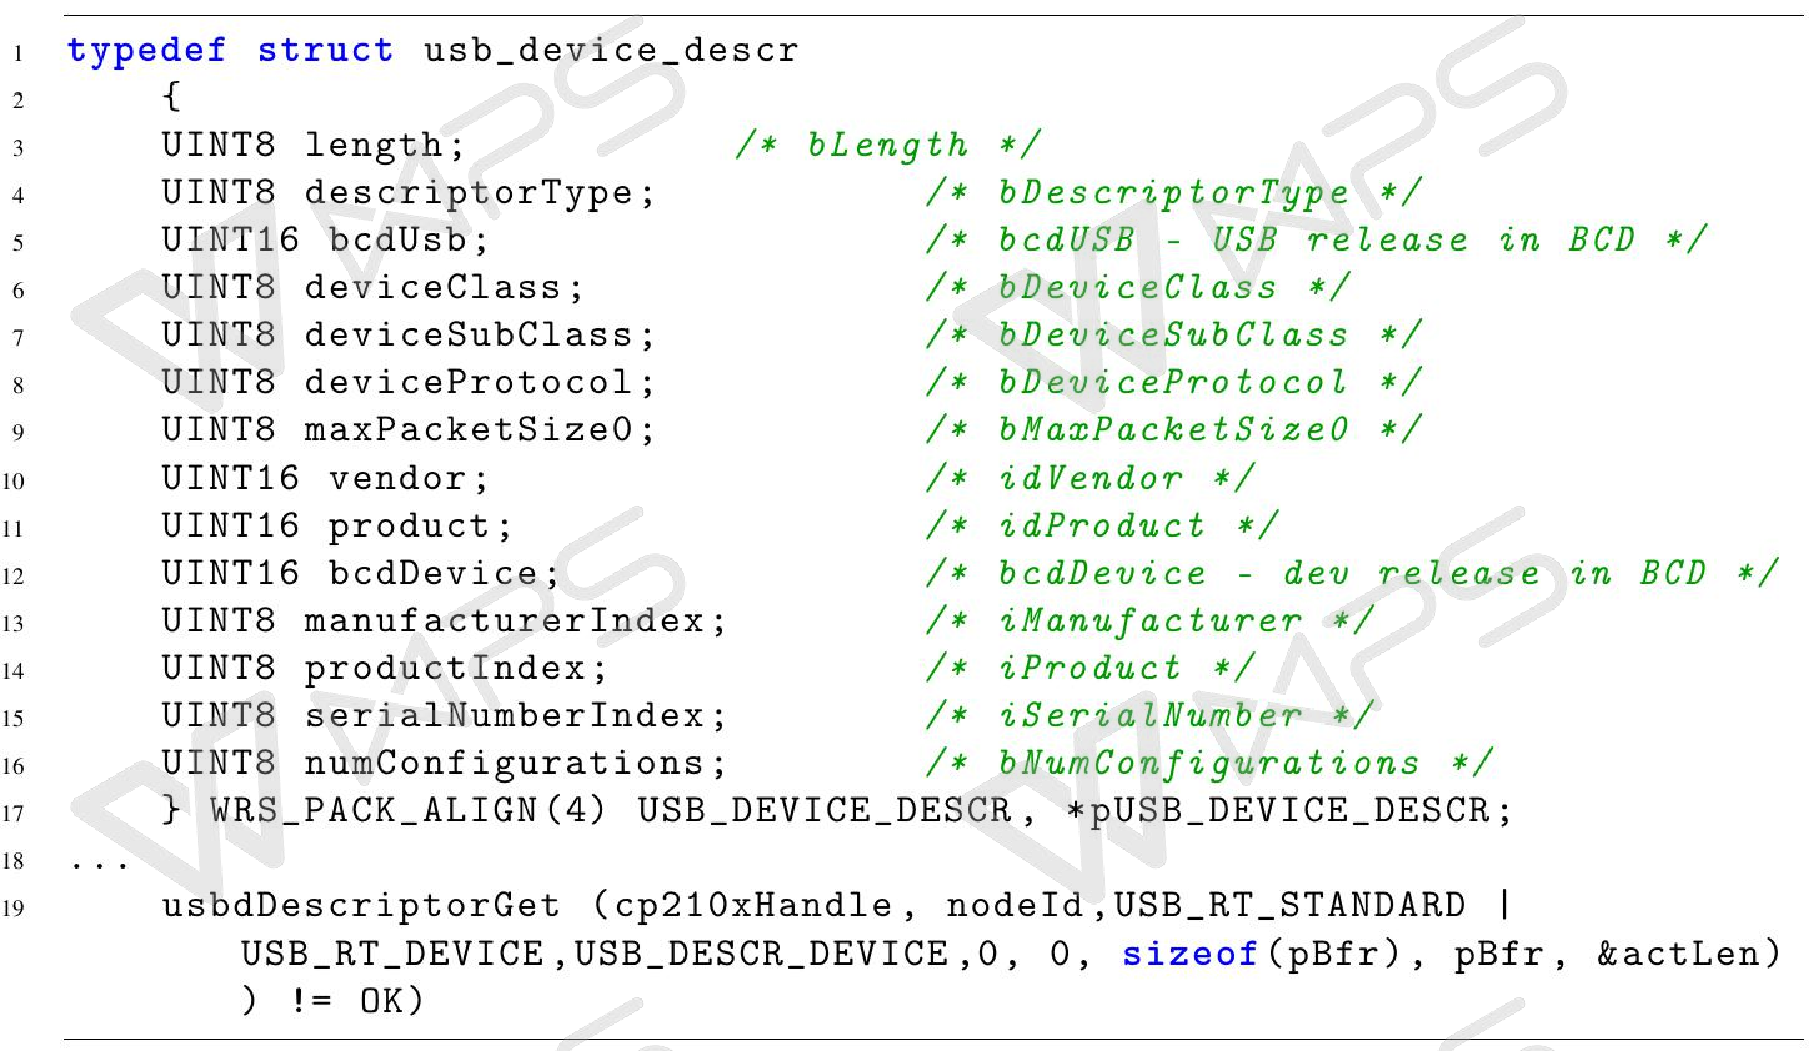
\includegraphics[width=1.0\textwidth]{./graphics/usdbDescriptorGet.pdf}
\caption{usb设备描述符信息结构}\label{fig:usdbDescriptorGet}
\end{figure}

使用usbdDescriptorGet()函数来获取设备描述符,其中第二、第三个参数是USB的标准请求命令,表示我们请求的是设备的标准描述符,获取到设备标准描述之后提取其中的厂商ID和产品ID,我们将该驱动支持的设备的厂商ID和设备ID存储在一个二维数组当中,然后通过遍历当前插入的设备的VID和PID是否在我们的数组当中来判断这个设备是否能够被我们的驱动所支持。设备识别的流程如\autoref{fig:device-recognize}所示,目前支持的设备的设备ID、产品ID的组合如\autoref{tab:目前支持的设备列表}所示。
\begin{figure}[!h]
\centering
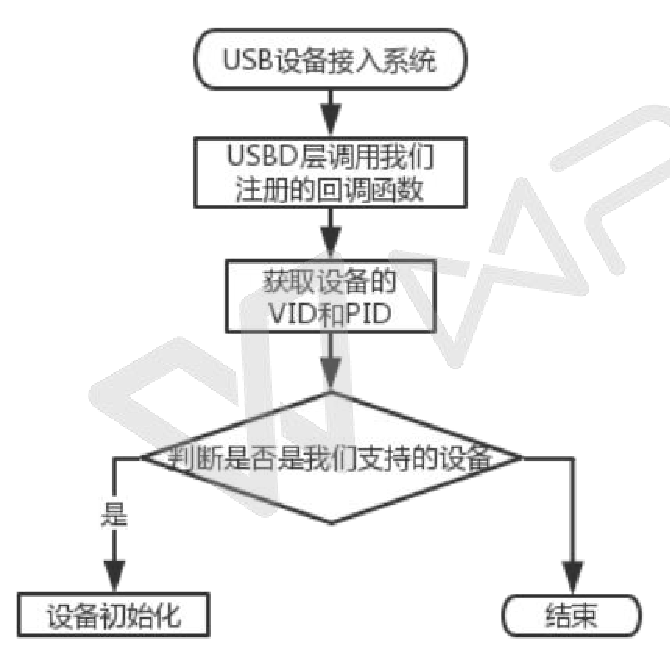
\includegraphics[width=.9\textwidth]{./graphics/device-recognize.pdf}
\caption{设备识别流程图}\label{fig:device-recognize}
\end{figure}

\begin{table}[!h]
\centering
\begin{tabular}{|c|c|c|c|c|c|c|}
\hline
{\hei{PID}}&{0x045B}&{0x0471}&{0x0489}&{0x0489}&{0x10C4}&{0x10C4}\\ 
\hline
{\hei{VID}}&{0x0053}&{0x066A}&{0xE000}&{0xE003}&{0x80F6}&{0x8115}\\
\hline 
{\hei{PID}}&{0x10C4}&{0x10C4}&{0x10C4}&{0x10C4}&{0x10C4}&{0x2405}\\
\hline
{\hei{VID}}&{0xEA60}&{0x813D}&{0x813F}&{0x814A}&{0x814B}&{0x0003}\\
\hline
\end{tabular}
\caption{目前支持的设备列表}\label{tab:目前支持的设备列表}
\end{table}

	
	
	



\subsection{设备的初始化}

	设备的初始化包括获取该USB设备的各种描述符信息。包括配置描述符信息、接口描述符信息、端点描述符信息。再通过所获得的这些信息来创建到输出端点的管道和对设备进行设置,我们在此处将设备的波特率初始化为115200,数据位为8位,1个停止位,没有奇偶校验,没有流控。设备的初始化流程图如\autoref{fig:device-init}所示。
\begin{figure}[!h]
\centering
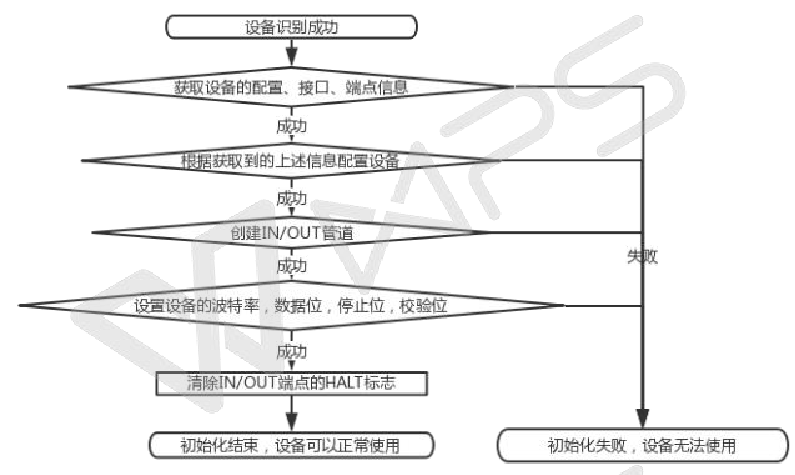
\includegraphics[width=1.0\textwidth]{./graphics/Dev-Init.pdf}
\caption{设备初始化流程图}\label{fig:device-init}
\end{figure}

这些描述符同样是通过usbdDescriptorGet()函数来发送设备的标准描述符命令来获取,在获取到
这些信息之后,通过usbdConfigurationSet()、usbdInterfaceSet()来配置设备,通过usbdPipeCreate()函数来设置设备的输入、输出管道,通过管道来连接设备的输入、输出端点。部分关键代码如下:
\lstset{language=C}
\begin{lstlisting}
...  
  usbdDescriptorGet (cp210xHandle, pCp210xDev->nodeId,USB_RT_STANDARD | USB_RT_DEVICE, USB_DESCR_CONFIGURATION,0, 0, USB_MAX_DESCR_LEN, pBfr, &actLen) 
  pCfgDescr = usbDescrParse (pBfr, actLen,USB_DESCR_CONFIGURATION)
  pScratchBfr = pBfr;
  ifNo = 0;
  while ((pIfDescr = usbDescrParseSkip (&pScratchBfr,&actLen,USB_DESCR_INTERFACE))!= NULL){
    if (ifNo == pCp210xDev->interface)
		break;
	ifNo++;
  }
  pOutEp = findEndpoint(pScratchBfr, actLen, USB_ENDPOINT_OUT)
  pInEp = findEndpoint(pScratchBfr,actLen,USB_ENDPOINT_IN))
...  
  usbdConfigurationSet (cp210xHandle, pCp210xDev->nodeId,pCfgDescr->configurationValue,pCfgDescr->maxPower * USB_POWER_MA_PER_UNIT)
...  
  usbdInterfaceSet(cp210xHandle,pCp210xDev->nodeId,pCp210xDev->interface,pIfDescr->alternateSetting);
...  
  usbdPipeCreate(cp210xHandle,pCp210xDev->nodeId,pOutEp->endpointAddress,pCfgDescr->configurationValue,pCp210xDev->interface,USB_XFRTYPE_BULK,USB_DIR_OUT,maxPacketSizeOut,0,0,&pCp210xDev->outPipeHandle)
...  
  usbdPipeCreate(cp210xHandle,pCp210xDev->nodeId,pInEp->endpointAddress,pCfgDescr->configurationValue,pCp210xDev->interface,USB_XFRTYPE_BULK,USB_DIR_IN,maxPacketSizeIn,0,0,&pCp210xDev->inPipeHandle)
...
\end{lstlisting}


\subsection{设备打开/关闭函数}

	用户在使用一个设备之前必须先对这个设备进行打开,在这个过程当中底层驱动的响应函数通常会将进行中断注册和使能设备工作配置等操作。但是对于我们的USB口转串口驱动而言,我们不需要自己管理中断,USBD层会为我们进行中断的管理工作,而配置工作我们在设备的初始化工作中已经完成,因此此处我们的设备打开工作,只需要简单的记录设备被打开的次数,并返回即可。设备的打开代码如下所示:
	
\lstset{language=C}
\begin{lstlisting}
LOCAL CP210X_DEV * cp210xDevOpen(DEV_HDR *pDevHdr, char *name, int flags,int mode)
{
	CP210X_DEV *pCp210xDev;
	pCp210xDev = (CP210X_DEV *)pDevHdr;
	if(!pCp210xDev->connected)	
		return (ERROR);
		
	(pCp210xDev->numOpen)++;
	return (pCp210xDev);
}
\end{lstlisting}

	第一个DEV\_ HDR类型的参数即是我们之前所说的必须是设备自定义结构的第一个成员,在此时它会由 IO 子系统自动提供,IO 子系统会根据驱动号寻址到对应驱动函数时,然后将对应的系统设备列表中存储的设备结构作为第一个参数来调用 cp210xDevOpen()。我们之后在使用的时候需要首先将这个 DEV\_ HDR 结构转换成我们的自定义结构 CP210X\_ DEV。但是我们也可以直接将第一个参数的类型设置为自定义结构类型,那么对于我们USB口转串口驱动,以上  cp210xDevOpen() 函数的调用原型就变为:LOCAL int cp210xDevOpen(CP210X\_ DEV *pCp210xDev, char *name, int flags,int mode)这并不会造成什么影响。
		
	第二个参数是设备名匹配后的剩余部分,注意不是我们传过来的设备名。VxWorks中使用最佳匹配的原则来匹配设备名,如我们打开一个设备"/ttyUsb/xyz",但是如果系统中并没有完全符合这个设备名的设备,而是只有名为"/ttyUsb/x"的设备,那么系统就会打开这个设备,而将匹配完成之后剩余的剩余的字符串"yz"传递给name。我们的应用中 open() 函数调用时的路径名应该与系统设备列表中的设备名是完全一致的,此处的 name 就会是一个空字符串,所以这个规则对于我们并没有什么影响。这是规则的主要用处在于处理文件系统层下的块设备,此处的name可以指向块设备节点名后的子目录和文件名。

	第三,四个参数就是用户 open() 调用时传入的第二,三个参数,IO 子系统不会对他们进行任何更改,只是原封不动的转发给了 cp210xDevOpen() 函数。
	
	该函数的返回值有如下两种值:一个有效的CP210X\_ DEV结构指针表示 cp210xDevOpen 调用成功,ERROR 则表示 cp210xDevOpen()调用失败,IO 子系统会根据返回的指针是否有效来决定返回一个文件描述符还是返回一个错误。cp210xDevOpen() 函数的返回值非常重要,这个指针将被 IO 子系统保存,用于其后对驱动中读写,控制函数的调用。这个返回的指针也会作为这些函数的第一个参数。
	
	设备的关闭和设备的打开操作是相反的操作,在关闭操作当中我们只需要对设备记录的打开次数进行减法操作即可。

\subsection{设备的读写}
	在open()操作成功之后,我们可以得到一个返回值,这个返回值就是设备的文件描述符,然后我们就可以使用这个文件描述符对设备进行read(),write()等操作。我们的USB口转串口驱动的读写函数原型如下:

\lstset{language=C}
\begin{lstlisting}
LOCAL int cp210xDevWrite(CP210X_DEV *pCp210xDev, char *buffer,UINT32 nBytes)
LOCAL int cp210xDevRead(CP210X_DEV *pCp210xDev, char *buffer,UINT32 nBytes)
\end{lstlisting}

此处我们将这两个函数的第一个参数类型直接设置为 CP210X\_ DEV 结构类型而不是DEV\_ HDR。
	在驱动的内部我们会为每一个连接到系统上的设备建立一个输入循环缓冲区和一个输出循环缓冲区,分别用于从设备接收的数据和接收上层应用的输出数据。缓存空间的大小作为以宏的方式定义在头文件当中,方便以后改动,分别定义为:WRITE\_ BUFFER\_ SIZE和READ\_ BUFFER\_ SIZE。
	
	由于我们特殊驱动程序的要求与普通流程下的驱动有所不同,其初始化方式比较特殊,对于数据的传输操作的流程也有相应的需求。我们在此需要对其数据流进行重新的设计。
	
	对于数据的输出若系统中没有连接上USB口转串口的设备时,那么所有的上层应用往外输出的数据就只会写入到输出循环缓冲区当中,	
	设备在连接上系统并初始化之后就先查询缓冲区中是否存在数据,若存在数据则将其发送,若不存在则等待其他程序调用write写入数据来触发数据的发送操作,系统调用write()在该驱动程序中对应的底层函数为cp210xDevWrite()函数,这个函数会接受write()发送过来的数据,并将其存入缓冲区中,并判断是否需要触发数据的发送操作。发送数据的触发操作只会在设备当前没有数据发送时完成,若调用write()时设备已经在发送数据,则只需要将数据存入缓冲区即可,设备发送完当前正在发送的数据之后会去判断缓冲区中是否还有数据,有数据则会继续发送。其流程图如\autoref{fig:outData-diagram} 所示。

\begin{figure}[!h]
\centering
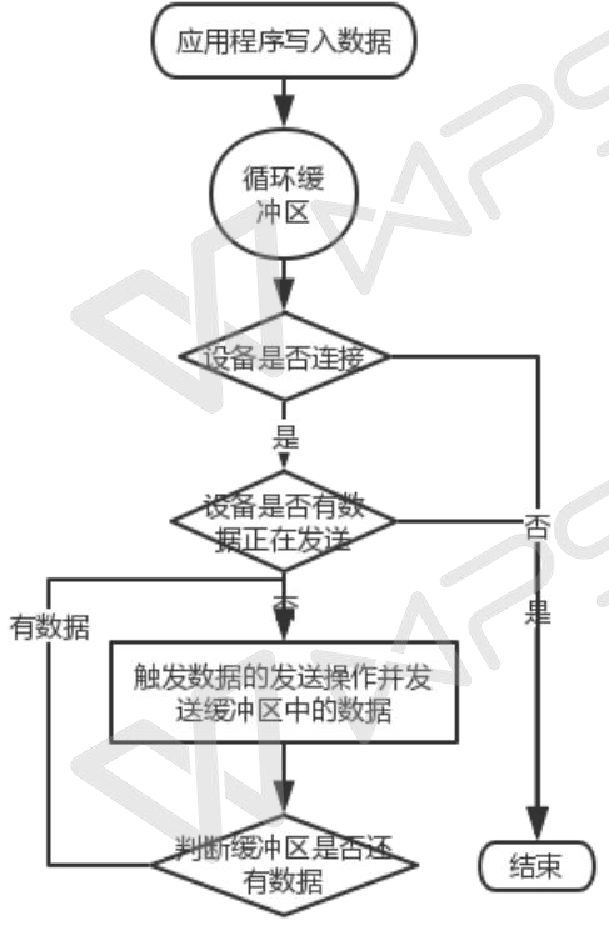
\includegraphics[width=.7\textwidth]{./graphics/data-send-diagram.pdf}
\caption{数据发送逻辑图}\label{fig:outData-diagram}
\end{figure}


	对于数据的输入操作,我们会事先创建好一个用来读取数据的USB IRP在这个IRP中我们注册一个回调函数,在USB当中设备的中断会由USBD层来替我们进行管理,当有数据到来时USBD层会调用我们注册的回调函数来通知我们。在驱动程序初始化完成之后我们就会启动listenForInput()这个函数来注册一个USBD的通知过程,一个接收IRP使用完成之后,我们需要重新注册一次,因为每一次的IRP都是单次有效的,所以在cp210xIrpCallback()中我们接受完这一次的IRP的数据之后, 需要新建另一个IRP重新启动下一次的listenForInput()过程。部分关键代码如下:
\lstset{language=C}
\begin{lstlisting}

LOCAL STATUS listenForInput(CP210X_DEV *pCp210xDev)
{
..
  pIrp->userPtr = pCp210xDev;
  pIrp->userCallback = cp210xIrpCallback;
  pIrp->timeout = USB_TIMEOUT_NONE;
  pIrp->transferLen = 64;
  if(usbdTransfer (cp210xHandle, pCp210xDev->inPipeHandle, pIrp) != OK)
...
}

LOCAL void cp210xIrpCallback(pVOID p)
{
...
	if(pIrp == &pCp210xDev->inIrp && pCp210xDev->connected == TRUE)
	{
		if(pIrp->result == OK)
			copy_to_readBuf(pCp210xDev);
			
		if (pIrp->result != S_usbHcdLib_IRP_CANCELED)
			listenForInput(pCp210xDev);
	}
}

\end{lstlisting}

	
	因为我们的驱动的程序的主要功能就在于数据的传输,在数据的传输过程中对于缓冲区的设计和信号量的使用方式直接影响到我们的驱动程序性能,因此有必要对这两部分再进行详细的描述。


\subsubsection{环形缓冲区的设计和实现}

	在我们的USB口转串口驱动程序当中 ,我们需要解决低速设备和处理器之间的速度匹配问题和数据丢失问题 ,这可以通过建立环形数据缓冲的方式来解决。当数据到达时,我们先将数据放入到缓冲区当中,当上层应用需要取出数据或者设备空闲了可以进行数据的发送工作的时候,我们再从缓冲区中将数据取出。
		
  应用程序、设备驱动和环形缓冲区的关系如\autoref{fig:设备数据缓冲}所示,通过环形数据缓冲,我们可以解决速度匹配的问题和数据丢失的问题,应用程序也无需阻塞等待设备的空闲,只需将数据发送到我们的缓冲区中即可。
  
\begin{figure}[!h]
\centering
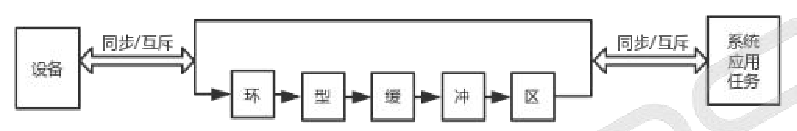
\includegraphics[width=.9\textwidth]{./graphics/Dev-Data-Buf.pdf}
\caption{设备数据缓冲}\label{fig:设备数据缓冲}
\end{figure}

	 
	我们使用循环队列实现的来实现环形缓冲区,由于计算机的内存是线性地址空间,因此从逻辑上实现环形缓冲区时通常需要4个指针:
	 \begin{itemize}
	 \item 在内存中实际开始位置的指针;
	 \item 在内存中实际结束位置的指针,或者缓冲区的长度,由于我们已经在缓冲区的头部定义了缓冲区的长度,所以这个指针我们不再需要;
	 \item 存储在缓冲区中的有效数据的开始位置(读指针);
	 \item 存储在缓冲区中的有效数据的结束位置的指针(写指针)。
	 \end{itemize}
	
当数据元素插入或者是删除时,我们不需要移动其余的数据元素存储位置,只需要移动队头和队尾指针即可。在设备初始化时,将设备的环形缓冲区清空,队头指针和队尾指针均设为 0,当缓冲区中接收到一个数据时,将此数据保存到队尾的位置并将队尾指针加1,当缓冲区中取走一个数据时,我们将队头指针减一。

	无论是对于读缓冲区还是写缓冲区,我们都需要解决的一个问题是当循环缓冲区中的数据已经满了之后,再有数据需要进入到缓冲区当中时,我们怎么进行处理,此处我们选择的策略是遵循先进先出的原则来覆盖数据。这样操作的好处是可以防止最新的数据丢失,而老的数据可能已经失去了时效性。

	对于输入缓冲区,我们使用一个读互斥信号量cp210xReadMutex和一个读二进制信号量ReadblockSem来进行缓冲区的控制,cp210xReadMutex的作用保证对读缓冲区的正确访问顺序,ReadblockSem的作用是用于对上层读任务和底层驱动的写任务进行同步。在使用ReadblockSem时我们会设置一个超时时间TIMEOUT,当时间超过时semTake()操作就会返回一个错误,我们上层读取任务此时就会得到一个错误返回,说明无法读取到数据。

\lstset{language=C}
\begin{lstlisting}
funA()//上层应用读取任务
{	
	semTake(cp210xReadMutex,WAIT_FOR_EVER)	
	if(available == 0)
	{
		semGive(cp210xReadMutex)
		//等待缓冲区写入数据,当底层往缓冲区中写入数据时会释放ReadblockSem
		status = semTake(ReadblockSem,TIEMOUT);
		if(status == ERROR)
			return ERROR;
			
		semTake(cp210xReadMutex,WAIT_FOR_EVER)
	}
	copy_from_readBuf; /*从缓冲区读取数据*/
	semGive(cp210xReadMutex)
	...
}

funB()//底层从硬件接收数据
{
	semTake(cp210xReadMutex,WAIT_FOR_EVER)
	if(available == 0)//缓冲区中没有数据,则释放一次ReadblockSem
		semGive(ReadblockSem);
	copy_to_readBuf()//向读缓冲区中写入数据
	semGive(cp210xReadMutex);
	
}
\end{lstlisting}  


	对于输出缓冲区,我们使用一个写互斥信号量cp210xWriteMutex来进行缓冲区的读写控制,由于我们这个特殊的驱动程序在往外输出数据时只需要将数据输出到了缓冲区的即可,不管实际的设备是否连接,因此我们不需要使用二进制信号量来进行上层写任务和底层读任务之间的同步操作。此时设备如果连接在系统上则会触发数据的发送操作,若设备没有连接在系统上,那么设备在连接上之后会自动的进行一次判断缓冲区中是否有数据的操作,有数据则触发发送操作。部分关键代码如下:

\lstset{language=C}
\begin{lstlisting}
funA()//上层应用写任务
{	
	semTake(cp210xWriteMutex,WAIT_FOR_EVER)	
	copy_to_writeBuf; /*从缓冲区读取数据*/
	semGive(cp210xWriteMutex)
	...
}

funB()//底层从缓冲区读取数据写入设备
{
	semTake(cp210xWriteMutex,WAIT_FOR_EVER)
	if(available == 0)
	{
		semGive(cp210xWriteMutex);
		return;
	}	
	copy_from_writeBuf()//向读缓冲区中写入数据
	initOutIrp();//构建数据发送IRP
	semGive(cp210xWriteMutex);
	...
}
\end{lstlisting}  

cp210xDevRead 和 cp210xDevWrite 的实现非常相似,只是更换了一下数据的传输方向。cp210xDevRead在底层也有一个循环缓冲区用来接收从USB口转串口设备发送来的数据,当需要读取 nbytes 个字节而缓冲区内的字节不够时,read就会阻塞,直到超时返回或者USBD层通知你有新的数据到来时再继续进行读操作。同时也在驱动中启动了一个计时器,如果在计时器时间到了之后,还未能满足需要读取的字节数,则退出本次读写操作,返回当前已处理的字节数。



\subsection{设备的控制操作}
	设备控制操作用于对设备的某一些工作行为进行再配置,可进行的在配置类别随着设备类型的不同而不同,操作系统当中通常会一种类型的设备的某一组共同属性作为一个配置选项,比如波特率再配置就是串口的一个标准属性,而一般的USB设备是不具有该属性的。但是这只是一个约定,并不是所有的设备都必须要完全对照这一准则,底层驱动也可以根据自己的实际需要来对这些再配置属性进行选择,我们可以选择只实现某一些再配置参数,也可以根据具体情况对某一个再配置选项进行响应,设备控制函数给用户控制设备提供方便的同时也对底层设备的实现提供了极大的方便性。
	
	对于我们的USB口转串口驱动而言,其属于一个特殊的设备,没法归入操作系统的已经分好类的设备当中,我们需要实现一些非约定的配置属性,如配置波特率、流控、数据位等等非USB所属的配置选项。
	我们将USB口转串口驱动特定的参数定义在一个头文件当中,而后将这个头文件提供给用户程序,当用户对设备进行操作时,其包含这个头文件,使用其中定义的特定参数对设备进行控制。IO 子系统不会对用户调用的ioctl()函数做任何的改变,只会将用户使用的选项参数或者控制命令传递给我们的cp210xDevIoctl()函数,然后由这个函数完成对选项参数或控制命令的解释和使用。
设备控制函数原型如下:
\lstset{language=C}
\begin{lstlisting}
LOCAL int cp210xDevIoctl(CP210X_DEV *pCp210xDev, int request, void *someArg )
\end{lstlisting}

对于我们的 USB口转串口驱动,在实际使用中,再配置参数和命令有很多,但是目前我们只提供设备的波特率、数据位、校验位、流控的参数和命令。这些控制对于普通的USB设备而言是没有的,他们在定义上属于USB的厂商自定义请求,在我们的驱动程序的cp210xDevIoctl()函数当中最后都要使用usbdVendorSpecific()函数来发送USB的厂商自定义请求,该函数的原型如\autoref{fig:usbdVendorSpecific}所示。


\begin{figure}[!h]
\centering
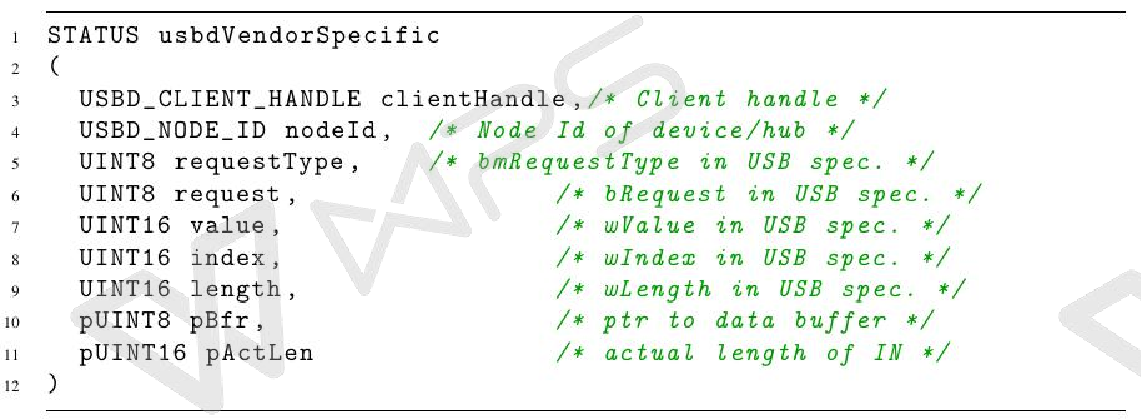
\includegraphics[width=1.0\textwidth]{./graphics/usbdVendorSpecify.pdf}
\caption{usbdVendorSpecific()}\label{fig:usbdVendorSpecific}
\end{figure}

其中第二个参数是请求类型,表示该类型是从主机到设备的,还是从设备到主机的,有四种类型,分别是REQTYPE\_ HOST\_ TO\_ INTERFACE(0x41),REQTYPE\_ INTERFACE\_ TO\_ HOST(0xC1),REQTYPE\_ HOST\_ TO\_ DEVICE(0x40),REQTYPE\_ DEVICE\_ TO\_ HOST((0xC0)),第三个参数是具体的请求,对于我们的设备而言能响应的部分主要请求如\autoref{fig:部分厂商自定义请求} 所示。

\begin{figure}[!h]
\centering
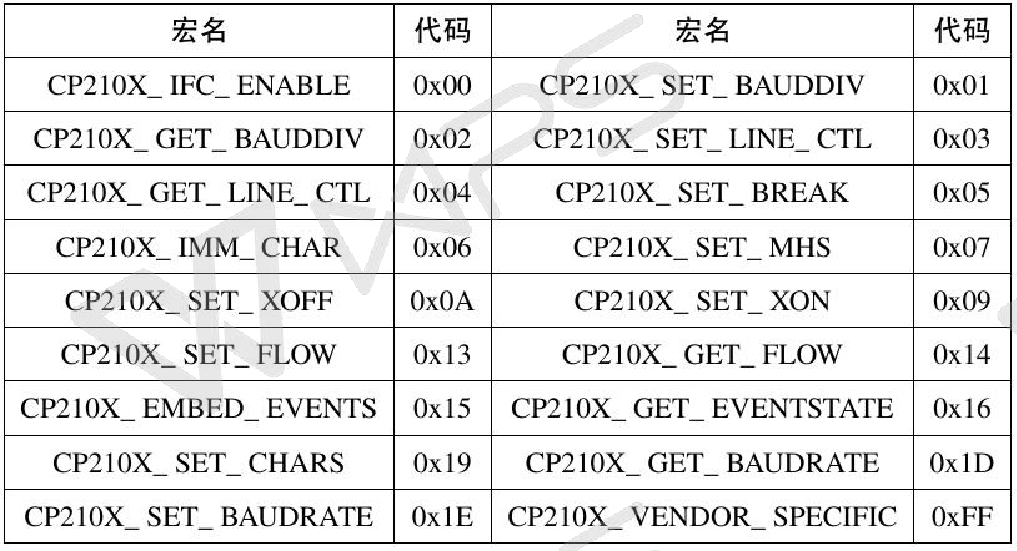
\includegraphics[width=1.0\textwidth]{./graphics/vendorSpecify.pdf}
\caption{部分厂商自定义请求}\label{fig:部分厂商自定义请求}
\end{figure}


\subsection{驱动卸载}
	在驱动的初始化函数cp210xDrvInit()当中我们使用了 iosDrvInstall() 函数向 IO 子系统注册我们的驱动,在wind中也提供了另外一个相反作用的函数iosDrvRemove()注销我们的驱动。该函数调用原型如\autoref{fig:iosDrvRemove}所示。
	
\begin{figure}[!h]
\centering
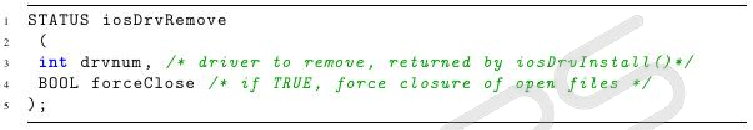
\includegraphics[width=1.0\textwidth]{./graphics/iosDrvRemove.pdf}
\caption{iosDrvRemove()}\label{fig:iosDrvRemove}
\end{figure}

该函数的第二个参数指定是否对驱动程序进行强制性的卸载,并将所有与此驱动有关的文件描述符关闭。如果强制关闭,则 IO 子系统将遍历系统文件描述符表,检查每个描述符对应结构中的驱动号是否等于要卸载驱动的驱动号,如果相同,则调用这个驱动的 close 实现函数进行关闭,同时释放文件描述符表中该表项,此时用户层的文件句柄将自动失去功效,如果用户其后使用这个文件描述符,将直接得到一个错误返回。

除了驱动卸载函数之外,我们的驱动初始化时还向USBD层进行了注册,在卸载的时候也应该注销USBD层的注册,同时注销动态注册的回调函数并从系统的设备表当中删除掉该设备。之后还应该对该驱动占用的所有其他的系统资源进行释放。



至此,我们已经完成了该特定需求下的USB口转串口驱动程序的所有组成部分的设计和实现。

\section{通用多设备驱动的实现}
多设备支持的驱动程序在初始化的时候与特定需求单设备支持的驱动初始化的过程是不一样的,需要支持多设备,首先需要在识别设备后给每一个设备分配一个设备名,并加入到系统设备表当中,然后需要给每一个设备初始化自己的设备结构体多设备下的驱动运行流程如\autoref{fig:MDev-Drv-diagram}所示。

\begin{figure}[p, !h]
\centering
  \begin{subfigure}[b]{1.0\textwidth}
  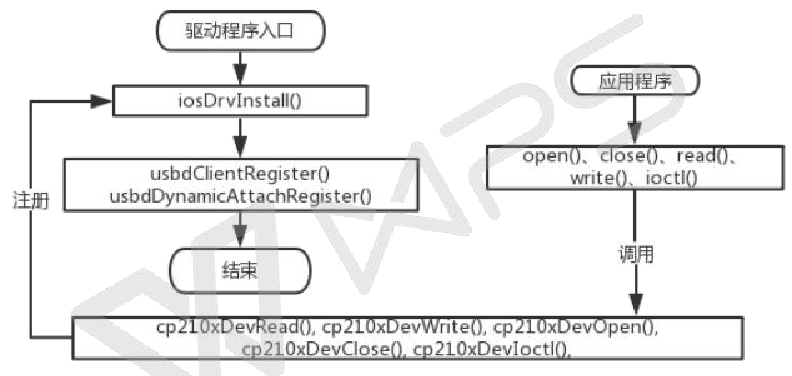
\includegraphics[width=\textwidth]{./graphics/MDev-Drv-Diagram-a.pdf}
  \caption{}\label{fig:MDevice-Driver-diagram-a}
  \end{subfigure}
  ~
  \begin{subfigure}[b]{1.0\textwidth}
  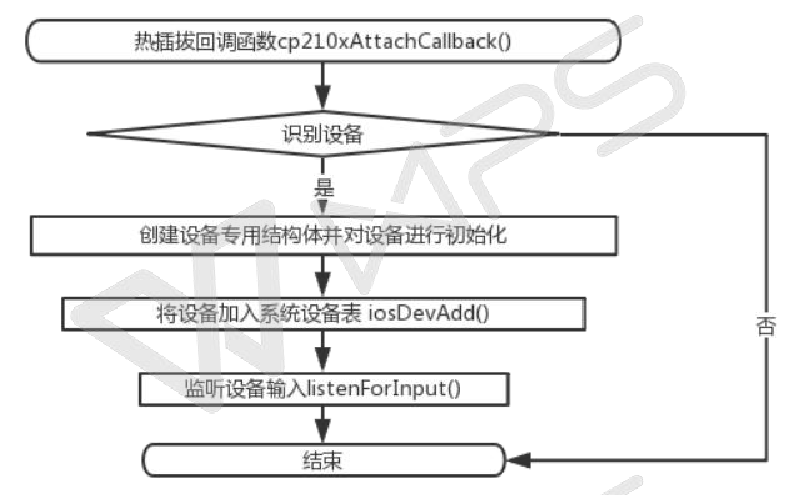
\includegraphics[width=\textwidth]{./graphics/MDev-Drv-Diagram-b.pdf}
  \caption{}\label{fig:MDevice-Driver-diagram-b}
  \end{subfigure}
\caption{多设备驱动运行流程图}\label{fig:MDev-Drv-diagram}
\end{figure}


与特定需求单设备的驱动相比,这里驱动程序的变化主要在驱动的初始化和读写函数部分,同时设备自定义的数据结构会更加复杂,需要保存更多与具体的设备相关的信息。

\subsection{设备的自定义结构体}
多设备的驱动自定义结构体的定义如下所示:
\lstset{language=C}
\begin{lstlisting}
typedef struct cp210x_dev
{
  DEV_HDR cp210xDevHdr; /*must be first field*/
  LINK 	devHdrLink; /*linked list of  devhdr structs*/
  UINT16 numOpen;
  USBD_NODE_ID nodeId; /*device nodeID*/
  UINT16 configuration; 
  UINT16 interface; /*a interface of this device*/
  UINT16 interfaceAltSetting;
  UINT16 vendorId;
  UINT16 productId;
  BOOL connected;
  
  int trans_len;
  USBD_PIPE_HANDLE outPipeHandle; /* USBD pipe handle for bulk OUT pipe*/
  USB_IRP	outIrp; /*IRP to monitor output to device*/
  BOOL outIrpInUse;
  UINT32 outErrors; /*TRUE while IRP is outstanding*/
  UINT8 trans_buf[64];
  UINT16  outEpAddr;  
  
  USBD_PIPE_HANDLE inPipeHandle;
  USB_IRP inIrp;
  BOOL inIrpInUse;
  UINT8 inBuf[64];
  UINT32 inErrors;
  UINT16 inEpAddr;
  
  char *writeBuf;
  int writeFront;
  int writeRear;
  char *readBuf;
  int readFront;
  int readRear;
} CP210X_DEV, *pCP210XDEV;
\end{lstlisting}
	在这个结构体当中我们增加了每个设备的读写缓冲区的指针和各个缓冲区的头尾指针。同时使用了一个链表devHdrLink来链接在系统上的由该驱动支持的设备,每次检测到新设备时我们可以通过将新添加的设备增加到这个链表当中,之后可以通过nodeId来从多个设备中定位我们的设备是否存在,之后我们可以给每一个设备分配一个设备名。部分代码如下所示:
\lstset{language=C}
\begin{lstlisting}
...
 usbListLinkProt(&devListHdr,(pVOID)pCp210xDev,(pLINK)&pCp210xDev->devHdrLink,LINK_TAIL,cp210xMutex);
...

LOCAL pCP210XDEV findDevHdr(USBD_NODE_ID nodeId)
{
	pCP210XDEV pCp210xDev =  usbListFirst(&devListHdr);

	while(pCp210xDev != NULL)
	{
		if(pCp210xDev->nodeId == nodeId)
			break;
		pCp210xDev = usbListNext(&pCp210xDev->devHdrLink);
	}
	return pCp210xDev;
}
\end{lstlisting}

\subsection{驱动注册和设备创建}

	比较单设备驱动初始化(如\autoref{fig:SDevice-Driver-diagram-a}所示)和多设备驱动初始化(如\autoref{fig:MDevice-Driver-diagram-a}所示),我们可以看出在驱动注册过程中两者的区别,在单设备驱动的初始化中我们先完成设备结构体的创建并定好一个设备名,之后直接将其加入到系统的设备表当中,即使此时没有设备连接。而在多设备的驱动初始化当中我们是在驱动的回调函数中驱动识别完了设备之后再完成设备结构体的创建和加入系统设备表的,这种方式是通用的设备驱动常采用的方式。
	在设备创建时我们会通过判断已连接设备的个数来决定当前设备所采用的设备名,部分代码如下:

\lstset{language=C}
\begin{lstlisting}
LOCAL int getCp210xDeviceNum(CP210X_DEV *pCp210xDev)
{
...
  for (int index=0; index < CP210X_MAX_DEVICE; index++)
    if (pCp210xDevArray[index] == NULL){
      pCp210xDevArray[index] = pCp210xDev;
      return (index);
    }
...
}
	
LOCAL STATUS cp210xAttachCallback(USBD_NODE_ID nodeId, UINT16 attachAction,UINT16 configuration,UINT16 interface,UINT16 deviceClass,UINT16 deviceSubClass, UINT16 deviceProtocol)
{
  ...
  cp210xUnitNum = getCp210xDeviceNum(pCp210xDev);
  sprintf (cp210xName, "%s%d", CP210X_NAME,cp210xUnitNum);
  if(iosDevAdd(&pCp210xDev->cp210xDevHdr,cp210xName,cp210xDrvNum) != OK)
  ...
}
\end{lstlisting}


\subsection{设备读写}
	
		
	对于通用多设备的写操作,与设定设备的操作不同的是设备连接上时,没有一个自动发送缓冲区的数据的过程,此时设备没有连接上也不可能往缓冲区中写入数据。其基本流程如下:	
	
	\begin{enumerate}
	\item 将数据拷贝到输出循环缓冲区当中。
	\item 判断设备是否处于连接状态。
	\item 若处于连接状态,那么是否有数据正在发送当中。若有数据正在发送,则无需操作。
	\item 若没有数据在发送,则触发发送数据的操作。
	\item 返回发送的字节数。
	\end{enumerate}
	
	
	对于数据发送的逻辑控制,我们使用一个互斥信号cp210xWriteMutex对输出缓冲区进行控制,首先在写入数据的时候需要进行互斥写,因为此时设备有可能正在从缓冲区当中取数据进行输出操作,那么这是写入输出缓冲区就需要等待,否则可能会造成缓冲区的混乱,造成输出结果与输入数据不一致。当设备输出从缓冲区拷贝完成之后就会释放互斥信号量,此时写入操作就可以往输出缓冲区中写入数据。
	
	
	多设备下的数据的输入  操作的实现方式与单设备下的相同, 都是在设备接入系统之后就向USBD层注册一个回调函数和一个IRP接收设备的输入,即listenForInput (),这个函数的实现与单设备驱动当中的一致,然后在cp210xIrpCallback()函数当中处理设备的输入,并启动下一次的listenForInput (),


	对于多设备情况下的驱动的其他部分如设备的控制、设备打开/关闭、设备卸载函数与单设备下的相比不需要做改变即可完成,此时操作的设备就是我们使用设备名打开的那个设备,IO子系统会将设备名映射到该设备所对应地驱动。





\section{小结}
	本章首先介绍了我们的USB口转串口驱动的设计想法,包括VxWorks下进行USB驱动开发的层次结构,USB口转串口所使用转换器的选择和对其进行开发工作所必须的知识。接下来我们讲解了我们的驱动程序的具体的设计和实现的方式,包括驱动中要实现的模块,每个模块的功能是什么,如何实现这些模块。



